\section{Detailed\_\-Items\_\-List  Class Reference}
\label{classDetailed__Items__List}\index{Detailed_Items_List@{Detailed\_\-Items\_\-List}}
{\tt \#include $<$dil2al.hh$>$}

Inheritance diagram for Detailed\_\-Items\_\-List::\begin{figure}[H]
\begin{center}
\leavevmode
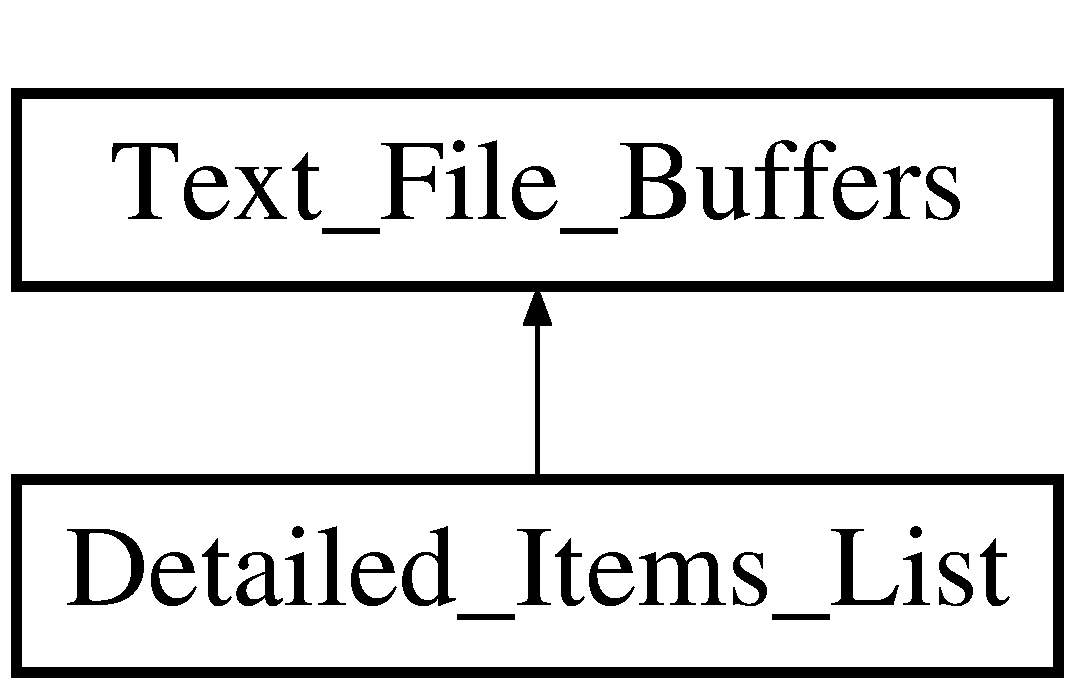
\includegraphics[height=2cm]{classDetailed__Items__List}
\end{center}
\end{figure}
\subsection*{Public Methods}
\begin{CompactItemize}
\item 
bool {\bf Entry\_\-Has\_\-Dependencies} (const {\bf DIL\_\-entry} $\ast$de, bool taggedonly={\bf false})
\item 
int {\bf Get\_\-Project\_\-Data} ({\bf String} \&dildata, int projloc, {\bf String} \&hrefurl, {\bf String} \&hreftext, {\bf DIL\_\-entry\_\-parameters} \&dilentrypars)
\item 
int {\bf Get\_\-All\_\-DIL\_\-ID\_\-File\_\-Parameters} ({\bf String} $\ast$dilid=NULL)
\item 
int {\bf Get\_\-All\_\-Topical\_\-DIL\_\-Parameters} (bool gettext={\bf false}, bool cacherefresh={\bf false})
\item 
{\bf DIL\_\-entry} $\ast$$\ast$ {\bf Sort\_\-by\_\-Target\_\-Date} (bool gettext={\bf false})
\item 
bool {\bf Write\_\-to\_\-File} ()
\item 
bool {\bf Binary\_\-Cache\_\-Diagnostic} ()
\end{CompactItemize}
\subsection*{Public Attributes}
\begin{CompactItemize}
\item 
{\bf PLLRoot}$<$ {\bf DIL\_\-entry} $>$ {\bf list}
\end{CompactItemize}
\subsection*{Protected Methods}
\begin{CompactItemize}
\item 
bool {\bf Write\_\-to\_\-Binary\_\-Cache} ()
\item 
bool {\bf Read\_\-from\_\-Binary\_\-Cache} ({\bf String} $\ast$dilid=NULL)
\item 
bool {\bf Write\_\-Topical\_\-to\_\-Binary\_\-Cache} (int diln, {\bf PLLRoot}$<$ {\bf DIL\_\-entry\_\-Pointer} $>$ \&dep, bool gottext)
\item 
bool {\bf Read\_\-Topical\_\-from\_\-Binary\_\-Cache} (int diln, bool gettext)
\end{CompactItemize}


\subsection{Member Function Documentation}
\index{Detailed_Items_List@{Detailed\_\-Items\_\-List}!Binary_Cache_Diagnostic@{Binary\_\-Cache\_\-Diagnostic}}
\index{Binary_Cache_Diagnostic@{Binary\_\-Cache\_\-Diagnostic}!Detailed_Items_List@{Detailed\_\-Items\_\-List}}
\subsubsection{\setlength{\rightskip}{0pt plus 5cm}bool Detailed\_\-Items\_\-List::Binary\_\-Cache\_\-Diagnostic ()}\label{classDetailed__Items__List_a6}




Definition at line 1643 of file utilities.cc.

References DIL\_\-entry::Binary\_\-Cache\_\-Diagnostic(), EOUT, Get\_\-All\_\-DIL\_\-ID\_\-File\_\-Parameters(), Get\_\-All\_\-Topical\_\-DIL\_\-Parameters(), PLLRoot$<$ DIL\_\-entry $>$::head(), PLLRoot$<$ DIL\_\-entry $>$::length(), list, PLLHandle$<$ DIL\_\-entry $>$::Next(), Read\_\-from\_\-Binary\_\-Cache(), Read\_\-Topical\_\-from\_\-Binary\_\-Cache(), VOUT, and Write\_\-to\_\-Binary\_\-Cache().

Referenced by Diagnostic().



\footnotesize\begin{verbatim}1643                                                   {
1644   // test if the quick load cache process works reliably
1645   VOUT << "dil2al::Detailed_Items_List::Binary_Cache_Diagnostic()\nTesting reliability of quick load cache process\n(Note that this is a good integrity test if modifications of the dilentry\nobjects necessitate corresponding modifications of the caching functions.)\n  flag `usequickloadcache' is ";
1646   if (usequickloadcache) VOUT << "set\n";
1647   else VOUT << "not set\n";
1648   // parse the HTML file
1649   bool _usequickloadcache = usequickloadcache;
1650   usequickloadcache = false;
1651   VOUT << "Parsing authoritative DIL parameters file\n";
1652   if (Get_All_DIL_ID_File_Parameters()<0) return false;
1653   VOUT << "Parsing authoritative DIL topical content files and writing to binary cache files\n";
1654   usequickloadcache = true;
1655   if (Get_All_Topical_DIL_Parameters(true,true)<0) return false;
1656   // save to cache
1657   VOUT << "Writing to binary cache file " << cacheidfile << '\n';
1658   if (!Write_to_Binary_Cache()) {
1659     EOUT << "dil2al: Unable to write to binary cache file " << cacheidfile << "in Detailed_Items_List::Binary_Cache_Diagnostic()\n";
1660     return false;
1661   }
1662   // load from cache into temporary list
1663   VOUT << "Reading from binary cache file into temporary list for comparison\n";
1664   Detailed_Items_List tmplist;
1665   if (!tmplist.Read_from_Binary_Cache()) return false;
1666   for (int n = 0; (dil[n]); n++) if (!tmplist.Read_Topical_from_Binary_Cache(n,true)) return false;
1667   // compare the original and temporary lists
1668   //   start of this object test
1669   int testedbytes = sizeof(Text_File_Buffers);
1670   VOUT << "Original length   = " << list.length() << '\n';
1671   VOUT << "Cache read length = " << tmplist.list.length() << '\n';
1672   testedbytes += sizeof(list);
1673   //   end of this object test
1674   if (testedbytes!=sizeof(Detailed_Items_List)) VOUT << "*** testedbytes!=sizeof(Detailed_Items_List)\n";
1675   for (DIL_entry * e = list.head(), * c = tmplist.list.head(); ((e) && (c)); e = e->Next(), c = c->Next()) if (!e->Binary_Cache_Diagnostic(c,testedbytes)) return false;
1676   VOUT << "Total bytes tested: " << testedbytes << '\n';
1677   usequickloadcache = _usequickloadcache;
1678   return true;
1679 }
\end{verbatim}\normalsize 
\index{Detailed_Items_List@{Detailed\_\-Items\_\-List}!Entry_Has_Dependencies@{Entry\_\-Has\_\-Dependencies}}
\index{Entry_Has_Dependencies@{Entry\_\-Has\_\-Dependencies}!Detailed_Items_List@{Detailed\_\-Items\_\-List}}
\subsubsection{\setlength{\rightskip}{0pt plus 5cm}bool Detailed\_\-Items\_\-List::Entry\_\-Has\_\-Dependencies (const {\bf DIL\_\-entry} $\ast$ {\em de}, bool {\em taggedonly} = {\bf false})}\label{classDetailed__Items__List_a0}




Definition at line 1131 of file utilities.cc.

References PLLRoot$<$ DIL\_\-entry $>$::head(), list, and PLL\_\-LOOP\_\-FORWARD.

Referenced by Tabbed\_\-FORM\_\-DIL\_\-Hierarchy\_\-full().



\footnotesize\begin{verbatim}1131                                                                                               {
1132   // if taggedonly==true then only dependencies with a set semaphore count
1133   if (!de) return false;
1134   if (taggedonly) {
1135     PLL_LOOP_FORWARD(DIL_entry,list.head(),1) if (e->Get_Semaphore()>0) if (e->Is_Direct_Dependency_Of(de)) return true;
1136   } else {
1137     PLL_LOOP_FORWARD(DIL_entry,list.head(),1) if (e->Is_Direct_Dependency_Of(de)) return true;
1138   }
1139   return false;
1140 }
\end{verbatim}\normalsize 
\index{Detailed_Items_List@{Detailed\_\-Items\_\-List}!Get_All_DIL_ID_File_Parameters@{Get\_\-All\_\-DIL\_\-ID\_\-File\_\-Parameters}}
\index{Get_All_DIL_ID_File_Parameters@{Get\_\-All\_\-DIL\_\-ID\_\-File\_\-Parameters}!Detailed_Items_List@{Detailed\_\-Items\_\-List}}
\subsubsection{\setlength{\rightskip}{0pt plus 5cm}int Detailed\_\-Items\_\-List::Get\_\-All\_\-DIL\_\-ID\_\-File\_\-Parameters ({\bf String} $\ast$ {\em dilid} = NULL)}\label{classDetailed__Items__List_a2}




Definition at line 1189 of file utilities.cc.

References absurl(), DIL\_\-AL\_\-List::al, String::at(), DIL\_\-AL\_\-List::bounded, DIL\_\-ID::chars(), PLLRoot$<$ DIL\_\-entry $>$::clear(), DIL\_\-Topical\_\-List::dil, EOUT, filetitle\_\-t::file, get\_\-file\_\-in\_\-list(), Get\_\-Project\_\-Data(), HTML\_\-get\_\-href(), HTML\_\-get\_\-table\_\-cell(), HTML\_\-remove\_\-comments(), String::index(), String::length(), PLLRoot$<$ DIL\_\-entry $>$::length(), PLLRoot$<$ DIL\_\-entry $>$::link\_\-before(), list, Big\-Regex::match\_\-info(), DIL\_\-entry::parameters, DIL\_\-AL\_\-List::priority, DIL\_\-entry::Projects(), Read\_\-from\_\-Binary\_\-Cache(), DIL\_\-AL\_\-List::relevance, DIL\_\-Topical\_\-List::relevance, String::SEARCH\_\-END, Big\-Regex::subpos(), DIL\_\-AL\_\-List::targetdate(), Text\_\-File\_\-Buffers::tf, Text\_\-File\_\-Buffers::tfname, Text\_\-File\_\-Buffers::tfnum, filetitle\_\-t::title, DIL\_\-entry\_\-parameters::topic\_\-append(), DIL\_\-entry::Topics(), DIL\_\-AL\_\-List::unbounded, DIL\_\-AL\_\-List::urgency, DIL\_\-ID::valid(), VOUT, and Write\_\-to\_\-Binary\_\-Cache().

Referenced by Binary\_\-Cache\_\-Diagnostic(), generate\_\-modify\_\-element\_\-FORM\_\-interface(), Get\_\-All\_\-Topical\_\-DIL\_\-Parameters(), modify\_\-DIL\_\-entry\_\-target\_\-date(), modify\_\-DIL\_\-group\_\-target\_\-dates(), modify\_\-element\_\-through\_\-FORM\_\-interface(), refresh\_\-quick\_\-load\_\-cache(), Tabbed\_\-DIL\_\-Hierarchy(), Tabbed\_\-FORM\_\-DIL\_\-Hierarchy(), Tabbed\_\-HTML\_\-DIL\_\-Hierarchy(), and update\_\-DIL\_\-entry\_\-elements().



\footnotesize\begin{verbatim}1189                                                                              {
1190 // Obtain parameters from the DIL by ID file for all DIL entries
1191 // or for the specific DIL entry dilid if dilid!=NULL
1192 // Note: deletes any previous linked list at listhead and refreshes
1193 // the DIL status
1194 
1195 /*
1196 INCREASING PARSING SPEED:
1197 
1198 A.
1199 
1200 To insure that the functionality is preserved, first properly comment each
1201 step done in the current version of the code.
1202 
1203 B.
1204 
1205 1. Can translate all A-Z characters to a-z to avoid capitalization issues.
1206 
1207 2. Can search for "<!--", then "-->", then test if find right tag between.
1208    You can also still use the Regex search here, since it is only one search.
1209 
1210 3. Can do the same for the end tag and copy that part of the text for parsing.
1211 
1212 4. Can find all chunks between <TR> <TR> and copy each to a separate String.
1213 
1214 5. Try to avoid Regex operations wherever possible.
1215 */
1216 
1217         if (Read_from_Binary_Cache(dilid)) return list.length();
1218 
1219         int ididx, idloc, entrynum = 0;
1220         if ((ididx=get_file_in_list(idfile,tf,tfname,tfnum))<0) return -1;
1221         if ((idloc=tf[ididx].index(BigRegex("[<]!--[    ]*dil2al:[      ]*DIL ID begin[         ]*--[>]"),String::SEARCH_END))<0) return -1;
1222         list.clear();
1223         // find next entry and obtain ID
1224         VOUT << "PARs: "; VOUT.flush();
1225         String idfilter("[^\"]*"); if (dilid) idfilter = (*dilid);
1226         BigRegex entryid(("[<]TR[>][^<]*[<]TD[>][^<]*[<]A[      ]+NAME[         ]*=[    ]*\"\\("+idfilter)+"\\)\"[^\n]*\n");
1227         while ((idloc=tf[ididx].index(entryid,String::SEARCH_END,idloc))>=0) {
1228                 int sp,ml;
1229                 if (!entryid.match_info(sp,ml,1)) {
1230                         EOUT << "dil2al: Missing ID in DIL entry " << entrynum << " in Detailed_Items_List::Get_All_DIL_ID_File_Parameters(), continuing\n";
1231                         continue;
1232                 }
1233                 DIL_entry * de = new DIL_entry(*this,tf[ididx].at(sp,ml)); // create candidate entry
1234                 if (!de->valid()) {
1235                         delete de;
1236                         EOUT << "dil2al: Invalid ID in DIL entry " << entrynum << " in Detailed_Items_List::Get_All_DIL_ID_File_Parameters(), continuing\n";
1237                         continue;
1238                 }
1239 #ifdef DIAGNOSTIC_OUTPUT
1240                 EOUT << "ID = " << de->chars() << '\n';
1241 #endif
1242                 // find comma separated list of topics
1243                 String topicline(tf[ididx].at(BigRegex("[<]TD[>][^\n]*\n"),idloc)); // topic data line
1244                 if (topicline.length()==0) {
1245                         delete de;
1246                         EOUT << "dil2al: Missing topical DIL reference in DIL entry " << entrynum << " in Detailed_Items_List::Get_All_DIL_ID_File_Parameters(), continuing\n";
1247                         continue;
1248                 }
1249                 idloc += topicline.length(); // position after data line
1250                 de->parameters = new DIL_entry_parameters(*de,entryid.subpos());
1251                 int topicloc = 0, numtopics = 0;
1252                 BigRegex entrytopic("\\([<]TD[>]\\|,\\)[^<]*[<]A[       ]+HREF[         ]*=[    ]*\"\\([^#]*\\)#[^\"]*\"[^>]*[>]\\([^<]*\\)[<]/A[>][    ]*(\\([^)]*\\))");
1253                 while ((topicloc=topicline.index(entrytopic,String::SEARCH_END,topicloc))>=0) {
1254                         int sp2, ml2, sp3, ml3;
1255                         if (!(entrytopic.match_info(sp,ml,2) && entrytopic.match_info(sp2,ml2,3) && entrytopic.match_info(sp3,ml3,4))) {
1256                                 EOUT << "dil2al: Invalid topical DIL reference in DIL entry " << entrynum << " in Detailed_Items_List::Get_All_Parameters(), continuing\n";
1257                                 continue;
1258                         }
1259                         de->parameters->topic_append(absurl(idfile,topicline.at(sp,ml)),topicline.at(sp2,ml2),atof(String(topicline.at(sp3,ml3))));
1260 #ifdef DIAGNOSTIC_OUTPUT
1261                         if (DIL_Topical_List * dtl = de->Topics(numtopics)) EOUT << "\ttopic file = " << dtl->dil.file << ", topic title = " << dtl->dil.title << "\n\t\trelevance = " << dtl->relevance << '\n';
1262 #endif
1263                         numtopics++;
1264                 }
1265                 if (!numtopics) {
1266                         delete de;
1267                         EOUT << "dil2al: Missing data in topical DIL field of DIL entry " << entrynum << " in Detailed_Items_List::Get_All_DIL_ID_File_Parameters(), continuing\n";
1268                         continue;
1269                 }
1270                 // find comma separated list of projects
1271                 int nextidloc; String cellparams, dildata;
1272                 if ((nextidloc=HTML_get_table_cell(tf[ididx],idloc,cellparams,dildata))<0) {
1273                         delete de;
1274                         EOUT << "dil2al: Missing project reference in DIL entry " << entrynum << " in Detailed_Items_List::Get_All_DIL_ID_File_Parameters(), continuing\n";
1275                         continue;
1276                 }
1277                 idloc = nextidloc;
1278                 HTML_remove_comments(dildata);
1279                 int projloc = 0, numprojects = 0; String hrefurl, hreftext;
1280                 while ((projloc=HTML_get_href(dildata,projloc,hrefurl,hreftext))>=0) {
1281                         int projidx;
1282                         hrefurl = absurl(idfile,hrefurl);
1283                         if ((projidx=Get_Project_Data(dildata,projloc,hrefurl,hreftext,*(de->parameters)))<0) {
1284                                 EOUT << "dil2al: Missing project data in DIL entry " << entrynum << " in Detailed_Items_List::Get_All_DIL_ID_File_Parameters(), continuing\n";
1285                                 continue;
1286                         }
1287                         projloc = projidx;
1288                         // (currently ignoring whether or not comma separates project references)
1289 #ifdef DIAGNOSTIC_OUTPUT
1290                         if (DIL_AL_List * dal = de->Projects(numprojects)) EOUT << "\tproject file = " << dal->al.file << ", project title = " << dal->al.title << "\n\t\trelevance = " << dal->relevance << ", unb.imp. = " << dal->unbounded << ", bound.imp. = " << dal->bounded << "\n\t\ttarget date = " << dal->targetdate() << ", urgency = " << dal->urgency << ", priority = " << dal->priority << '\n';
1291 #endif
1292                         numprojects++;
1293                 }
1294 // *** Currently we tolerate missing project related data
1295 /*              if (!numprojects) {
1296                         delete de;
1297                         EOUT << "dil2al: Missing data in project reference of DIL entry " << entrynum << " in Detailed_Items_List::Get_All_Parameters(), continuing\n";
1298                         continue;
1299                 }
1300 */
1301                 // attach to list
1302                 list.link_before(de);
1303                 entrynum++;
1304                 if ((entrynum % 10)==0) { VOUT << '.'; VOUT.flush(); }
1305         }
1306         VOUT << '\n'; VOUT.flush();
1307 #ifdef DIAGNOSTIC_OUTPUT
1308         EOUT << "Number of entries = " << entrynum << '\n';
1309 #endif
1310 
1311         if (!Write_to_Binary_Cache()) EOUT << "dil2al: Unable to write to binary cache file " << cacheidfile << "in Detailed_Items_List::Get_All_DIL_ID_File_Parameters(), continuing as is\n";
1312 
1313         return entrynum;
1314 }
\end{verbatim}\normalsize 
\index{Detailed_Items_List@{Detailed\_\-Items\_\-List}!Get_All_Topical_DIL_Parameters@{Get\_\-All\_\-Topical\_\-DIL\_\-Parameters}}
\index{Get_All_Topical_DIL_Parameters@{Get\_\-All\_\-Topical\_\-DIL\_\-Parameters}!Detailed_Items_List@{Detailed\_\-Items\_\-List}}
\subsubsection{\setlength{\rightskip}{0pt plus 5cm}int Detailed\_\-Items\_\-List::Get\_\-All\_\-Topical\_\-DIL\_\-Parameters (bool {\em gettext} = {\bf false}, bool {\em cacherefresh} = {\bf false})}\label{classDetailed__Items__List_a3}




Definition at line 1316 of file utilities.cc.

References DIL\_\-ID::chars(), PLLRoot$<$ PLLType $>$::clear(), DIL\_\-entry\_\-content::completion, DIL\_\-entry::content, DIL\_\-entry::elbyid(), EOUT, Get\_\-All\_\-DIL\_\-ID\_\-File\_\-Parameters(), DIL\_\-entry::Get\_\-Entry\_\-Parameters(), get\_\-file\_\-in\_\-list(), PLLRoot$<$ DIL\_\-entry $>$::head(), HTML\_\-get\_\-name(), HTML\_\-get\_\-table\_\-cell(), HTML\_\-get\_\-table\_\-row(), HTML\_\-remove\_\-tags(), PLLRoot$<$ DIL\_\-entry $>$::length(), PLLRoot$<$ PLLType $>$::link\_\-before(), list, PLL\_\-LOOP\_\-FORWARD, Read\_\-Topical\_\-from\_\-Binary\_\-Cache(), DIL\_\-entry\_\-content::required, String::SEARCH\_\-END, DIL\_\-entry\_\-content::started, DIL\_\-entry\_\-content::text, Text\_\-File\_\-Buffers::tf, Text\_\-File\_\-Buffers::tfname, Text\_\-File\_\-Buffers::tfnum, DIL\_\-entry\_\-content::valuation, VOUT, and Write\_\-Topical\_\-to\_\-Binary\_\-Cache().

Referenced by Binary\_\-Cache\_\-Diagnostic(), generate\_\-modify\_\-element\_\-FORM\_\-interface(), refresh\_\-quick\_\-load\_\-cache(), Sort\_\-by\_\-Target\_\-Date(), Tabbed\_\-DIL\_\-Hierarchy(), Tabbed\_\-FORM\_\-DIL\_\-Hierarchy(), and Tabbed\_\-HTML\_\-DIL\_\-Hierarchy().



\footnotesize\begin{verbatim}1316                                                                                                        {
1317 // Obtain parameters from the Topical DIL files for all DIL entries
1318 // Note: calls Get_All_DIL_ID_File_Parameters() if necessary
1319 // to link data to a linked list of DIL entries
1320 // *** could add options to either overwrite prior data
1321 //     (current state) or skip duplicate occurrances
1322   int ididx,idloc,entrynum,topicalentrynum = 0;
1323   PLLRoot<DIL_entry_Pointer> dep; // used to note DIL entries per cache
1324   if (!list.head()) entrynum=Get_All_DIL_ID_File_Parameters();
1325   else entrynum=list.length();
1326   VOUT << "DILs: "; VOUT.flush();
1327   for (int n=0; (dil[n]); n++) {
1328     if ((usequickloadcache) && (!cacherefresh)) if (Read_Topical_from_Binary_Cache(n,gettext)) continue;
1329 
1330     dep.clear();
1331     if ((ididx=get_file_in_list(*(dil[n]),tf,tfname,tfnum))<0) return -1;
1332     if ((idloc=tf[ididx].index(BigRegex("[<]!--[        ]*dil2al:[      ]*DIL begin[    ]*--[>]"),String::SEARCH_END))<0) return -1;
1333     // find next entry and obtain ID
1334     DIL_ID dilid; String markparams, rowcontent, cellcontent, reftext; int rowloc,cellloc, topicalDILentrynum = 0;
1335     while ((idloc=HTML_get_table_row(tf[ididx],idloc,markparams,rowcontent))>=0) {
1336       if ((rowloc=HTML_get_table_cell(rowcontent,0,markparams,cellcontent))<0) {
1337         EOUT << "dil2al: Missing DIL ID in " << *(dil[n]) << " at entry " << topicalDILentrynum << " in Get_All_Topical_DIL_Parameters()\n";
1338         return -1;
1339       }
1340       if ((cellloc=HTML_get_name(cellcontent,0,markparams,reftext))<0) {
1341         EOUT << "dil2al: Missing DIL ID name in " << *(dil[n]) << " at entry " << topicalDILentrynum << " in Get_All_Topical_DIL_Parameters()\n";
1342         return -1;
1343       }
1344       dilid = markparams; // obtain DIL entry ID
1345       DIL_entry * de;
1346       if ((de = list.head()->elbyid(dilid))==NULL) { // find ID in DIL
1347         EOUT << "dil2al: DIL ID " << dilid.chars() << " in " << *(dil[n]) << " not found in " << idfile << " in Get_All_Topical_DIL_Parameters()\n";
1348 //#define FIND_DILID_LIST_ERROR
1349 #ifdef FIND_DILID_LIST_ERROR
1350         EOUT << "List of DIL entries:\n";
1351         PLL_LOOP_FORWARD(DIL_entry,list.head(),1) EOUT << e->chars() << '\n';
1352 #endif
1353         return -1;
1354       }
1355       // obtain parameters
1356       if ((rowloc=HTML_get_table_cell(rowcontent,rowloc,markparams,cellcontent))<0) {
1357         EOUT << "dil2al: Missing parameters in " << *(dil[n]) << " at entry " << topicalDILentrynum << " in Get_All_Topical_DIL_Parameters()\n";
1358         return -1;
1359       }
1360       HTML_remove_tags(cellcontent);
1361       if (!de->Get_Entry_Parameters(cellcontent)) {
1362         EOUT << "dil2al: Invalid entry parameters in " << *(dil[n]) << " at entry " << topicalDILentrynum << " in Get_All_Topical_DIL_Parameters()\n";
1363         return -1;
1364       }
1365       // obtain text
1366       if ((idloc=HTML_get_table_row(tf[ididx],idloc,markparams,rowcontent))<0) {
1367         EOUT << "dil2al: Missing DIL text row in " << *(dil[n]) << " at entry " << topicalDILentrynum << " in Get_All_Topical_DIL_Parameters()\n";
1368         return -1;
1369       }
1370       if (gettext) {
1371         if ((rowloc=HTML_get_table_cell(rowcontent,0,markparams,cellcontent))<0) {
1372           EOUT << "dil2al: Missing DIL text in " << *(dil[n]) << " at entry " << topicalDILentrynum << " in Get_All_Topical_DIL_Parameters()\n";
1373           return -1;
1374         }
1375         //HTML_remove_comments(cellcontent);
1376         if (!de->content) de->content = new DIL_entry_content(*de);
1377         delete de->content->text; // remove prior allocation
1378         de->content->text = new String(cellcontent);
1379       }
1380 #ifdef DIAGNOSTIC_OUTPUT
1381       EOUT << "ID = " << de->chars() << " (" << de->content->started << ',' << de->content->required << ',' << de->content->completion << ',' << de->content->valuation << ")\n";
1382 #endif
1383       if (usequickloadcache) dep.link_before(new DIL_entry_Pointer(de));
1384       topicalDILentrynum++;
1385     }
1386 
1387     if (!Write_Topical_to_Binary_Cache(n,dep,gettext)) EOUT << "dil2al: Unable to write topical to binary cache file " << dil.File(n)->chars() << ".cache in Detailed_Items_List::Get_All_Topical_DIL_Parameters(), continuing as is\n";
1388 
1389     topicalentrynum += topicalDILentrynum;
1390     VOUT << '#'; VOUT.flush();
1391   }
1392   VOUT << '\n'; VOUT.flush();
1393 #ifdef DIAGNOSTIC_OUTPUT
1394   EOUT << "Number of topical entries = " << topicalentrynum << '\n';
1395 #endif
1396   return entrynum;
1397 }
\end{verbatim}\normalsize 
\index{Detailed_Items_List@{Detailed\_\-Items\_\-List}!Get_Project_Data@{Get\_\-Project\_\-Data}}
\index{Get_Project_Data@{Get\_\-Project\_\-Data}!Detailed_Items_List@{Detailed\_\-Items\_\-List}}
\subsubsection{\setlength{\rightskip}{0pt plus 5cm}int Detailed\_\-Items\_\-List::Get\_\-Project\_\-Data ({\bf String} \& {\em dildata}, int {\em projloc}, {\bf String} \& {\em hrefurl}, {\bf String} \& {\em hreftext}, {\bf DIL\_\-entry\_\-parameters} \& {\em dilentrypars})}\label{classDetailed__Items__List_a1}




Definition at line 1142 of file utilities.cc.

References String::at(), String::del(), DILSUPS\_\-TDPROP\_\-FIXED, find\_\-delimiter(), String::index(), String::length(), DIL\_\-entry\_\-parameters::project\_\-append(), and time\_\-stamp\_\-time().

Referenced by Get\_\-All\_\-DIL\_\-ID\_\-File\_\-Parameters().



\footnotesize\begin{verbatim}1142                                                                                                                                                  {
1143 // dildata contains the DIL entry project data
1144 // projloc indicates how much of dildata has already been parsed
1145 // hrefurl and hreftext have already been obtained
1146 // dilentrypars receives the DIL entry project related parameters
1147 // *** Modify this if the data format changes
1148         int nextproj, dataloc, dataend;
1149         // insure prior to next project URL
1150         if ((nextproj = dildata.index('<',projloc))<0) nextproj=dildata.length();
1151         // start of project data
1152         if ((dataloc = find_delimiter(dildata,projloc,nextproj,'('))<0) return -1;
1153         dataloc++;
1154         // find relevance data
1155         if ((dataend = find_delimiter(dildata,dataloc,nextproj,','))<0) return -1;
1156         double relevance = atof(String(dildata.at(dataloc,dataend-dataloc)));
1157         dataloc=dataend+1;
1158         // find unbounded importance data
1159         if ((dataend = find_delimiter(dildata,dataloc,nextproj,','))<0) return -1;
1160         double unbounded = atof(String(dildata.at(dataloc,dataend-dataloc)));
1161         dataloc=dataend+1;
1162         // find bounded importance data
1163         if ((dataend = find_delimiter(dildata,dataloc,nextproj,','))<0) return -1;
1164         double bounded = atof(String(dildata.at(dataloc,dataend-dataloc)));
1165         dataloc=dataend+1;
1166         // find target date and target date properties
1167         if ((dataend = find_delimiter(dildata,dataloc,nextproj,','))<0) return -1;
1168         String ymdHM = dildata.at(dataloc,dataend-dataloc);
1169         int tdprop = 0;
1170         if ((ymdHM.length()>0) && (ymdHM[0]=='F')) {
1171                 tdprop = DILSUPS_TDPROP_FIXED;
1172                 ymdHM.del(0,1);
1173         }
1174         if (ymdHM.length()<12) ymdHM += "0000"; // year, month, day, hour, minute
1175         time_t targetdate = time_stamp_time(ymdHM); // local time stamp stored in calendar time
1176         dataloc=dataend+1;
1177         // find urgency data
1178         if ((dataend = find_delimiter(dildata,dataloc,nextproj,','))<0) return -1;
1179         double urgency = atof(String(dildata.at(dataloc,dataend-dataloc)));
1180         dataloc=dataend+1;
1181         // find priority data
1182         if ((dataend = find_delimiter(dildata,dataloc,nextproj,')'))<0) return -1;
1183         double priority = atof(String(dildata.at(dataloc,dataend-dataloc)));
1184         // store project data
1185         dilentrypars.project_append(hrefurl,hreftext,relevance,unbounded,bounded,targetdate,tdprop,urgency,priority);
1186         return dataend+1;
1187 }       
\end{verbatim}\normalsize 
\index{Detailed_Items_List@{Detailed\_\-Items\_\-List}!Read_from_Binary_Cache@{Read\_\-from\_\-Binary\_\-Cache}}
\index{Read_from_Binary_Cache@{Read\_\-from\_\-Binary\_\-Cache}!Detailed_Items_List@{Detailed\_\-Items\_\-List}}
\subsubsection{\setlength{\rightskip}{0pt plus 5cm}bool Detailed\_\-Items\_\-List::Read\_\-from\_\-Binary\_\-Cache ({\bf String} $\ast$ {\em dilid} = NULL)\hspace{0.3cm}{\tt  [protected]}}\label{classDetailed__Items__List_b1}




Definition at line 1487 of file utilities.cc.

References PLLRoot$<$ DIL\_\-entry $>$::clear(), DILBYID\_\-CACHE\_\-NUMENTRIES\_\-SUSPICIOUS, EOUT, PLLRoot$<$ DIL\_\-entry $>$::link\_\-before(), list, Lock\_\-File(), DIL\_\-entry::Read\_\-from\_\-Binary\_\-Cache(), READSOMETYPE, res, DIL\_\-ID::str(), Unlock\_\-File(), and VOUT.

Referenced by Binary\_\-Cache\_\-Diagnostic(), and Get\_\-All\_\-DIL\_\-ID\_\-File\_\-Parameters().



\footnotesize\begin{verbatim}1487                                                                       {
1488   // Read a binary copy of the DIL parameters list from a cache file for quick loading.
1489   if (!usequickloadcache) return false;
1490   if (!Lock_File(lockidfile,idfile+" locked by Detailed_Items_List::Read_from_Binary_Cache()\n")) return false;
1491   if (verbose) VOUT << "Reading parameters from binary cache file\n";
1492   bool res = true;
1493   // read and compare CRC for idfile
1494   int retstat;
1495   if ((retstat=system("cksum "+idfile+" > "+crcidfile+".tmp"))==-1) {
1496     EOUT << "dil2al: Unable to check CRC in Detailed_Items_List::Read_from_Binary_Cache()\n";
1497     res = false;
1498   } else {
1499     retstat = (((retstat) & 0xff00) >> 8);
1500     VOUT << "retstat = " << retstat << '\n';
1501     if ((retstat=system("diff -q "+crcidfile+" "+crcidfile+".tmp"))!=0) {
1502       res = false;
1503       if (verbose) VOUT << "CRC difference - parsing of authoritative parameter file forced\n";
1504     }
1505     retstat = (((retstat) & 0xff00) >> 8);
1506     VOUT << "retstat = " << retstat << '\n';
1507     if (unlink(crcidfile+".tmp")<0) EOUT << "Unable to remove temporary CRC file " << crcidfile << ".tmp in Detailed_Items_List::Read_from_Binary_Cache(), continuing as is\n";
1508   }
1509   if (res) { // read parameters from binary cache file
1510     ifstream cfl(cacheidfile,ios::binary);
1511     if (!cfl) {
1512       EOUT << "dil2al: Unable to read from " << cacheidfile << " in Detailed_Items_List::Read_from_Binary_Cache()\n";
1513       res=false;
1514     } else {
1515       list.clear();
1516       int numentries, numentriesread = 0;
1517       if ((cfl.read((READSOMETYPE) (&numentries),sizeof(numentries))).gcount()<sizeof(numentries)) res = false;
1518 #ifdef TEST_CACHE_READ
1519       VOUT << "&&& numentries = " << numentries << '\n'; cout.flush();
1520 #endif
1521       while (res) {
1522 #ifdef TEST_CACHE_READ
1523         VOUT << "&&& numentriesread = " << numentriesread << '\n'; cout.flush();
1524 #endif
1525         DIL_entry * de = new DIL_entry(*this);
1526         if (!de->Read_from_Binary_Cache(cfl)) { 
1527           delete de;
1528           if (numentriesread<numentries) {
1529             EOUT << "dil2al: WARNING - Insufficient data retrieved from binary cache file in Detailed_Items_List::Read_from_Binary_Cache()\n";
1530             res = false;
1531           }
1532           break;
1533         }
1534         if (dilid) {
1535                 if (de->str()==(*dilid)) list.link_before(de); else delete de;
1536         } else list.link_before(de);
1537         numentriesread++;
1538         if (numentriesread>numentries) {
1539           EOUT << "dil2al: WARNING - Actual amount of data exceeds cached DIL length retrieved from binary cache file in Detailed_Items_List::Read_from_Binary_Cache()\n";
1540           res = false;
1541         }
1542       }
1543       cfl.close();
1544       if ((res) && (numentriesread<DILBYID_CACHE_NUMENTRIES_SUSPICIOUS)) {
1545         EOUT << "dil2al: Number of cached entries read (" << numentriesread << ") deemed suspiciously few, parsing of authoritative parameter file forced\n";
1546         res = false;
1547       }
1548     }
1549   }
1550   if (!Unlock_File(lockidfile)) EOUT << "dil2al: Unable to remove lock file " << lockidfile << " in Detailed_Items_List::Read_from_Binary_Cache(), continuing as is\n";
1551   return res;
1552 }
\end{verbatim}\normalsize 
\index{Detailed_Items_List@{Detailed\_\-Items\_\-List}!Read_Topical_from_Binary_Cache@{Read\_\-Topical\_\-from\_\-Binary\_\-Cache}}
\index{Read_Topical_from_Binary_Cache@{Read\_\-Topical\_\-from\_\-Binary\_\-Cache}!Detailed_Items_List@{Detailed\_\-Items\_\-List}}
\subsubsection{\setlength{\rightskip}{0pt plus 5cm}bool Detailed\_\-Items\_\-List::Read\_\-Topical\_\-from\_\-Binary\_\-Cache (int {\em diln}, bool {\em gettext})\hspace{0.3cm}{\tt  [protected]}}\label{classDetailed__Items__List_b3}




Definition at line 1554 of file utilities.cc.

References DIL\_\-ID::chars(), DIL\_\-entry::elbyid(), EOUT, PLLRoot$<$ DIL\_\-entry $>$::head(), list, Lock\_\-File(), DIL\_\-ID::Read\_\-DIL\_\-ID\_\-from\_\-Binary\_\-Cache(), DIL\_\-entry::Read\_\-Topical\_\-from\_\-Binary\_\-Cache(), READSOMETYPE, res, Unlock\_\-File(), and VOUT.

Referenced by Binary\_\-Cache\_\-Diagnostic(), and Get\_\-All\_\-Topical\_\-DIL\_\-Parameters().



\footnotesize\begin{verbatim}1554                                                                                {
1555   // Read a binary copy of the DIL Topical content from a cache file for quick loading.
1556   if (!usequickloadcache) return false;
1557   String filename((*dil.File(diln)));
1558   String lockfile(filename+".lock"), cachefile(filename+".cache"), crcfile(filename+".crc");
1559   if (!Lock_File(lockfile,filename+" locked by Detailed_Items_List::Read_Topical_from_Binary_Cache()\n")) return false;
1560   if (verbose) VOUT << "Reading topical content from binary cache file\n";
1561   bool res = true;
1562   // read and compare CRC for filename
1563   if (system("cksum "+filename+" > "+crcfile+".tmp")==-1) {
1564     EOUT << "dil2al: Unable to check CRC in Detailed_Items_List::Read_Topical_from_Binary_Cache()\n";
1565     res = false;
1566   } else {
1567     if (system("diff -q "+crcfile+" "+crcfile+".tmp")!=0) {
1568       res = false;
1569       if (verbose) VOUT << "CRC difference - parsing of authoritative topical content file forced\n";
1570     }
1571     if (unlink(crcfile+".tmp")<0) EOUT << "Unable to remove temporary CRC file " << crcfile << ".tmp in Detailed_Items_List::Read_Topical_from_Binary_Cache(), continuing as is\n";
1572   }
1573   if (res) { // read parameters from binary cache file
1574     ifstream cfl(cachefile,ios::binary);
1575     if (!cfl) {
1576       EOUT << "dil2al: Unable to read from " << cachefile << " in Detailed_Items_List::Read_Topical_from_Binary_Cache()\n";
1577       res=false;
1578     } else {
1579       bool gottext;
1580       if ((cfl.read((READSOMETYPE) (&gottext),sizeof(gottext))).gcount()<sizeof(gottext)) res = false;
1581       int numentries, numentriesread = 0;
1582       if ((cfl.read((READSOMETYPE) (&numentries),sizeof(numentries))).gcount()<sizeof(numentries)) res = false;
1583 #ifdef TEST_CACHE_READ
1584       VOUT << "&&& numentries = " << numentries << '\n'; cout.flush();
1585 #endif
1586       if ((gettext) && (!gottext)) {
1587         VOUT << "Text content needed and not available in cache, parsing of authoritative topical content file forced\n";
1588         res = false;
1589       }
1590       while (res) {
1591 #ifdef TEST_CACHE_READ
1592         VOUT << "&&& numentriesread = " << numentriesread << '\n'; cout.flush();
1593 #endif
1594         DIL_ID did;
1595         if (!did.Read_DIL_ID_from_Binary_Cache(cfl)) {
1596           if (numentriesread<numentries) {
1597             EOUT << "dil2al: WARNING - Insufficient data retrieved from binary cache file in Detailed_Items_List::Read_Topical_from_Binary_Cache()\n";
1598             res = false;
1599           }
1600           break;
1601         } else {
1602 #ifdef TEST_CACHE_READ
1603           VOUT << "&&& did = " << did.chars() << '\n'; cout.flush();
1604 #endif
1605           DIL_entry * de = list.head()->elbyid(did);
1606 #ifdef TEST_CACHE_READ
1607           VOUT << "&&& de = " << de->chars() << '\n'; cout.flush();
1608 #endif
1609           if (!de) {
1610             EOUT << "dil2al: DIL ID " << did.chars() << " not found in Detailed_Items_List::Read_Topical_from_Binary_Cache()\n";
1611             res = false;
1612           } else {
1613 #ifdef TEST_CACHE_READ
1614             VOUT << "&&& de->Read_Topical_from_Binary_Cache(cfl," << gottext << ")\n"; cout.flush();
1615 #endif
1616             if (!de->Read_Topical_from_Binary_Cache(cfl,gottext)) { 
1617               EOUT << "dil2al: Unable to read topical content for " << did.chars() << " in Detailed_Items_List::Read_Topical_from_Binary_Cache()\n";
1618               res = false;
1619             } else {
1620               /*            if (dilid) {
1621                             if (de->str()==(*dilid)) list.link_before(de); else delete de;
1622                             } else list.link_before(de); */
1623               numentriesread++;
1624               if (numentriesread>numentries) {
1625                 EOUT << "dil2al: WARNING - Actual amount of data exceeds cached DIL length retrieved from binary cache file in Detailed_Items_List::Read_Topical_from_Binary_Cache()\n";
1626                 res = false;
1627               }
1628             }
1629           }
1630         }
1631       }
1632       cfl.close();
1633       if ((res) && (numentriesread<1)) {
1634         EOUT << "dil2al: Number of cached entries read (" << numentriesread << ") deemed suspiciously few, parsing of authoritative topical content file forced\n";
1635         res = false;
1636       }
1637     }
1638   }
1639   if (!Unlock_File(lockfile)) EOUT << "dil2al: Unable to remove lock file " << lockfile << " in Detailed_Items_List::Read_Topical_from_Binary_Cache(), continuing as is\n";
1640   return res;
1641 }
\end{verbatim}\normalsize 
\index{Detailed_Items_List@{Detailed\_\-Items\_\-List}!Sort_by_Target_Date@{Sort\_\-by\_\-Target\_\-Date}}
\index{Sort_by_Target_Date@{Sort\_\-by\_\-Target\_\-Date}!Detailed_Items_List@{Detailed\_\-Items\_\-List}}
\subsubsection{\setlength{\rightskip}{0pt plus 5cm}{\bf DIL\_\-entry} $\ast$$\ast$ Detailed\_\-Items\_\-List::Sort\_\-by\_\-Target\_\-Date (bool {\em gettext} = {\bf false})}\label{classDetailed__Items__List_a4}




Definition at line 1681 of file utilities.cc.

References DIL\_\-entry\_\-target\_\-date\_\-qsort\_\-compare(), EOUT, Get\_\-All\_\-Topical\_\-DIL\_\-Parameters(), PLLRoot$<$ DIL\_\-entry $>$::head(), PLLRoot$<$ DIL\_\-entry $>$::length(), list, and PLL\_\-LOOP\_\-FORWARD.

Referenced by modify\_\-DIL\_\-group\_\-target\_\-dates(), select\_\-TL\_\-DIL\_\-refs(), stop\_\-TL\_\-chunk(), and update\_\-DIL\_\-to\_\-AL().



\footnotesize\begin{verbatim}1681                                                                           {
1682 // Create an array of pointers to DIL entries and sort it in
1683 // ascending order of target dates
1684         int entrynum,i = 0;
1685         if (!list.head()) entrynum=Get_All_Topical_DIL_Parameters(gettext);
1686         else entrynum=list.length();
1687         if (entrynum<1) {
1688                 EOUT << "dil2al: No DIL to sort in Detailed_Items_List::Sort_by_Target_Date()\n";
1689                 return NULL;
1690         }
1691         // set up array
1692         DIL_entry ** dep = new (DIL_entry *)[entrynum];
1693         PLL_LOOP_FORWARD(DIL_entry,list.head(),(i<entrynum)) { dep[i] = e; i++; }
1694         // sort array
1695         qsort(dep,entrynum,sizeof(DIL_entry *),DIL_entry_target_date_qsort_compare);
1696         return dep;
1697 }
\end{verbatim}\normalsize 
\index{Detailed_Items_List@{Detailed\_\-Items\_\-List}!Write_to_Binary_Cache@{Write\_\-to\_\-Binary\_\-Cache}}
\index{Write_to_Binary_Cache@{Write\_\-to\_\-Binary\_\-Cache}!Detailed_Items_List@{Detailed\_\-Items\_\-List}}
\subsubsection{\setlength{\rightskip}{0pt plus 5cm}bool Detailed\_\-Items\_\-List::Write\_\-to\_\-Binary\_\-Cache ()\hspace{0.3cm}{\tt  [protected]}}\label{classDetailed__Items__List_b0}




Definition at line 1416 of file utilities.cc.

References EOUT, PLLRoot$<$ DIL\_\-entry $>$::head(), PLLRoot$<$ DIL\_\-entry $>$::length(), list, Lock\_\-File(), PLL\_\-LOOP\_\-FORWARD, res, Unlock\_\-File(), and VOUT.

Referenced by Binary\_\-Cache\_\-Diagnostic(), and Get\_\-All\_\-DIL\_\-ID\_\-File\_\-Parameters().



\footnotesize\begin{verbatim}1416                                                 {
1417   // Write a binary copy of the DIL parameters list to a cache file for quick loading.
1418   bool res = true;
1419   if (usequickloadcache) {
1420     if (Lock_File(lockidfile,idfile+" locked by Detailed_Items_List::Write_to_Binary_Cache()\n")) {
1421       if (verbose) VOUT << "Writing parameters to binary cache file\n";
1422       ofstream cfl(cacheidfile,ios::binary);
1423       if (!cfl) {
1424         EOUT << "dil2al: Unable to write to " << cacheidfile << " in Detailed_Items_List::Write_to_Binary_Cache()\n";
1425         res=false;
1426       } else {
1427         int numentries = list.length();
1428         cfl.write((const void *) (&numentries),sizeof(numentries));
1429         PLL_LOOP_FORWARD(DIL_entry,list.head(),1) if (!e->Write_to_Binary_Cache(cfl)) { res=false; break; }
1430         cfl.close();
1431       }
1432       // write new CRC for idfile and unlock
1433       if (res) if (system("cksum "+idfile+" > "+crcidfile)==-1)  EOUT << "dil2al: Unable to write new CRC to " << crcidfile << " in Detailed_Items_List::Write_to_Binary_Cache(), continuing as is\n";
1434       if (!Unlock_File(lockidfile)) EOUT << "dil2al: Unable to remove lock file " << lockidfile << " in Detailed_Items_List::Write_to_Binary_Cache(), continuing as is\n";
1435     } else {
1436       EOUT << "dil2al: Unable to prepare a Quick Load Cache in Detailed_Items_List::Write_to_Binary_Cache()\n";
1437       res=false;
1438     }
1439   }
1440   return res;
1441 }
\end{verbatim}\normalsize 
\index{Detailed_Items_List@{Detailed\_\-Items\_\-List}!Write_to_File@{Write\_\-to\_\-File}}
\index{Write_to_File@{Write\_\-to\_\-File}!Detailed_Items_List@{Detailed\_\-Items\_\-List}}
\subsubsection{\setlength{\rightskip}{0pt plus 5cm}bool Detailed\_\-Items\_\-List::Write\_\-to\_\-File ()}\label{classDetailed__Items__List_a5}




Definition at line 1699 of file utilities.cc.

References String::at(), String::before(), String::chars(), DILBYID\_\-FLOAT\_\-FORMAT, DILSUPS\_\-BND\_\-UNSPECIFIED, DILSUPS\_\-PRI\_\-UNSPECIFIED, DILSUPS\_\-REL\_\-UNSPECIFIED, DILSUPS\_\-TD\_\-UNSPECIFIED, DILSUPS\_\-TDPROP\_\-FIXED, DILSUPS\_\-UNB\_\-UNSPECIFIED, DILSUPS\_\-URG\_\-UNSPECIFIED, DILTOPICS\_\-REL\_\-UNSPECIFIED, EOUT, Text\_\-File\_\-Buffers::File\-Index(), PLLRoot$<$ DIL\_\-entry $>$::head(), HTML\_\-get\_\-table\_\-row(), HTML\_\-marker\_\-arguments(), HTML\_\-put\_\-href(), HTML\_\-put\_\-name(), HTML\_\-put\_\-table\_\-cell(), HTML\_\-put\_\-table\_\-row(), String::length(), list, DIL\_\-entry::parameters, PLL\_\-LOOP\_\-FORWARD, PLL\_\-LOOP\_\-FORWARD\_\-NESTED, relurl(), String::SEARCH\_\-END, Text\_\-File\_\-Buffers::tf, time\_\-stamp(), and write\_\-file\_\-from\_\-String().

Referenced by modify\_\-DIL\_\-entry\_\-target\_\-date(), modify\_\-DIL\_\-group\_\-target\_\-dates(), and update\_\-DIL\_\-entry\_\-parameter\_\-elements().



\footnotesize\begin{verbatim}1699                                         {
1700 // writes a modified DIL-by-ID file
1701 // requires that Topic and Project/Superior parameters are available
1702 // (such as provided by a prior call to Get_All_DIL_ID_File_Parameters())
1703 #ifdef CAUTIOUS_OBJECT_INTERFACES
1704         int ididx = FileIndex(idfile);
1705         if (ididx<0) return false;
1706 #else
1707         const int ididx = 0;
1708 #endif
1709         // copy free-style header and table column headings
1710         int idloc;
1711         if ((idloc=tf[ididx].index(BigRegex("[<]!--[    ]*dil2al:[      ]*DIL ID begin[         ]*--[>]"),String::SEARCH_END))<0) {
1712                 EOUT << "dil2al: Missing header in " << idfile << " in Detailed_Items_List::Write_to_File(), continuing as is\n";
1713                 return false;
1714         }
1715         String newidfile(tf[ididx].through(idloc)), rowparams, rowcontent;
1716         idloc = HTML_get_table_row(tf[ididx],idloc,rowparams,rowcontent);
1717         rowparams = HTML_marker_arguments(rowparams);
1718         newidfile += "\n\n" + HTML_put_table_row(rowparams,rowcontent,true);
1719         // generate table
1720         DIL_entry * de = list.head();
1721         if (!de) {
1722                 EOUT << "dil2al: No DIL entries in list to write to " << idfile << " in Detailed_Items_List::Write_to_File(), continuing as is\n";
1723                 return false;
1724         }
1725         if (de->parameters) {
1726                 String topics, projects, tstamp;
1727                 PLL_LOOP_FORWARD(DIL_entry,de,1) {
1728                         topics = ""; PLL_LOOP_FORWARD_NESTED(DIL_Topical_List,e->Topics(0),1,te) {
1729                                 if (topics.length()>0) topics += ", ";
1730                                 topics += HTML_put_href(relurl(idfile,te->dil.file)+'#'+e->chars(),te->dil.title)+" (";
1731                                 if (te->relevance==DILTOPICS_REL_UNSPECIFIED) topics += "?.?)";
1732                                 else topics += String(te->relevance,DILBYID_FLOAT_FORMAT)+')';
1733                         }
1734                         if (topics.length()<=0) {
1735                                 topics = "@MISSING TOPICAL CONTENT REFERENCE@";
1736                                 EOUT << "dil2al: Warning - missing Topical Content Reference for DIL#" << e->chars() << " in " << idfile << " in Detailed_Items_List::Write_to_File(), continuing\n";
1737                         }
1738                         projects = ""; PLL_LOOP_FORWARD_NESTED(DIL_AL_List,e->Projects(0),1,pe) {
1739                                 if (projects.length()>0) projects += ", ";
1740                                 projects += HTML_put_href(relurl(idfile,pe->al.file),pe->al.title)+" (";
1741                                 if (pe->relevance==DILSUPS_REL_UNSPECIFIED) projects += "?.?,";
1742                                 else projects += String(pe->relevance,DILBYID_FLOAT_FORMAT)+',';
1743                                 if (pe->unbounded==DILSUPS_UNB_UNSPECIFIED) projects += "?.?,";
1744                                 else projects += String(pe->unbounded,DILBYID_FLOAT_FORMAT)+',';
1745                                 if (pe->bounded==DILSUPS_BND_UNSPECIFIED) projects += "?.?,";
1746                                 else projects += String(pe->bounded,DILBYID_FLOAT_FORMAT)+',';
1747                                 if (pe->tdproperty()==DILSUPS_TDPROP_FIXED) projects += 'F';
1748                                 if (pe->targetdate()==DILSUPS_TD_UNSPECIFIED) projects += "?,";
1749                                 else {
1750                                         tstamp = time_stamp("%Y%m%d%H%M",pe->targetdate());
1751                                         if (tstamp.at((int) tstamp.length()-4,4)=="0000") tstamp = tstamp.before((int) tstamp.length()-4);
1752                                         projects += tstamp+',';
1753                                 }
1754                                 if (pe->urgency==DILSUPS_URG_UNSPECIFIED) projects += "?.?,";
1755                                 else projects += String(pe->urgency,DILBYID_FLOAT_FORMAT)+',';
1756                                 if (pe->priority==DILSUPS_PRI_UNSPECIFIED) projects += "?.?)";
1757                                 else projects += String(pe->priority,DILBYID_FLOAT_FORMAT)+')';
1758                         }
1759                         if (projects.length()<=0) projects = "&nbsp;";
1760                         newidfile += HTML_put_table_row("",'\n'+HTML_put_table_cell("",HTML_put_name(e->chars(),e->chars()),true)+'\n'+
1761                                                                                 HTML_put_table_cell("",topics,true)+'\n'+
1762                                                                                 HTML_put_table_cell("",projects,true),true)+"\n\n";
1763                 }
1764         }
1765         // copy free-style footer
1766         if ((idloc=tf[ididx].index(BigRegex("[<]!--[    ]*dil2al:[      ]*DIL ID end[   ]*--[>]"),idloc))<0) {
1767                 EOUT << "dil2al: Missing footer in " << idfile << " in Detailed_Items_List::Write_to_File(), continuing as is\n";
1768                 return false;
1769         }
1770         newidfile += tf[ididx].from(idloc);
1771         return write_file_from_String(idfile,newidfile,"DIL ID");
1772 }
\end{verbatim}\normalsize 
\index{Detailed_Items_List@{Detailed\_\-Items\_\-List}!Write_Topical_to_Binary_Cache@{Write\_\-Topical\_\-to\_\-Binary\_\-Cache}}
\index{Write_Topical_to_Binary_Cache@{Write\_\-Topical\_\-to\_\-Binary\_\-Cache}!Detailed_Items_List@{Detailed\_\-Items\_\-List}}
\subsubsection{\setlength{\rightskip}{0pt plus 5cm}bool Detailed\_\-Items\_\-List::Write\_\-Topical\_\-to\_\-Binary\_\-Cache (int {\em diln}, {\bf PLLRoot}$<$ {\bf DIL\_\-entry\_\-Pointer} $>$ \& {\em dep}, bool {\em gottext})\hspace{0.3cm}{\tt  [protected]}}\label{classDetailed__Items__List_b2}




Definition at line 1443 of file utilities.cc.

References EOUT, PLLRoot$<$ PLLType $>$::head(), PLLRoot$<$ PLLType $>$::length(), Lock\_\-File(), PLL\_\-LOOP\_\-FORWARD, res, Unlock\_\-File(), and VOUT.

Referenced by Get\_\-All\_\-Topical\_\-DIL\_\-Parameters().



\footnotesize\begin{verbatim}1443                                                                                                                 {
1444   // Write a binary copy of the DIL parameters list to a cache file for quick loading.
1445   /*
1446     the structure in each cached topical content file is:
1447     bool gottext
1448     int DILentrynum
1449     for each entry:
1450       DIL_ID dilid
1451       bool hascontent
1452       time_t started
1453       time_t required
1454       float completion
1455       float valuation
1456       int textlen
1457       char[] text
1458   */
1459   bool res = true;
1460   if (usequickloadcache) {
1461     String filename((*dil.File(diln)));
1462     String lockfile(filename+".lock"), cachefile(filename+".cache"), crcfile(filename+".crc");
1463     if (Lock_File(lockfile,filename+" locked by Detailed_Items_List::Write_Topical_to_Binary_Cache()\n")) {
1464       if (verbose) VOUT << "Writing topical content to binary cache file\n";
1465       ofstream cfl(cachefile,ios::binary);
1466       if (!cfl) {
1467         EOUT << "dil2al: Unable to write to " << cachefile << " in Detailed_Items_List::Write_Topical_to_Binary_Cache()\n";
1468         res=false;
1469       } else {
1470         cfl.write((const void *) (&gottext),sizeof(gottext));
1471         int DILentrynum = dep.length();
1472         cfl.write((const void *) (&DILentrynum),sizeof(DILentrynum));
1473         PLL_LOOP_FORWARD(DIL_entry_Pointer,dep.head(),1) if (!e->Entry()->Write_Topical_to_Binary_Cache(cfl,gottext)) { res=false; break; }
1474         cfl.close();
1475       }
1476       // write new CRC for filename and unlock
1477       if (res) if (system("cksum "+filename+" > "+crcfile)==-1)  EOUT << "dil2al: Unable to write new CRC to " << crcfile << " in Detailed_Items_List::Write_topical_to_Binary_Cache(), continuing as is\n";
1478       if (!Unlock_File(lockfile)) EOUT << "dil2al: Unable to remove lock file " << lockfile << " in Detailed_Items_List::Write_Topical_to_Binary_Cache(), continuing as is\n";
1479     } else {
1480       EOUT << "dil2al: Unable to prepare a Quick Load Cache in Detailed_Items_List::Write_Topical_to_Binary_Cache()\n";
1481       res=false;
1482     }
1483   }
1484   return res;
1485 }
\end{verbatim}\normalsize 


\subsection{Member Data Documentation}
\index{Detailed_Items_List@{Detailed\_\-Items\_\-List}!list@{list}}
\index{list@{list}!Detailed_Items_List@{Detailed\_\-Items\_\-List}}
\subsubsection{\setlength{\rightskip}{0pt plus 5cm}{\bf PLLRoot}$<${\bf DIL\_\-entry}$>$ Detailed\_\-Items\_\-List::list}\label{classDetailed__Items__List_m0}




Definition at line 706 of file dil2al.hh.

Referenced by Binary\_\-Cache\_\-Diagnostic(), Entry\_\-Has\_\-Dependencies(), exit\_\-report(), generate\_\-modify\_\-element\_\-FORM\_\-interface(), Get\_\-All\_\-DIL\_\-ID\_\-File\_\-Parameters(), Get\_\-All\_\-Topical\_\-DIL\_\-Parameters(), modify\_\-DIL\_\-entry\_\-target\_\-date(), modify\_\-DIL\_\-group\_\-target\_\-dates(), modify\_\-DIL\_\-group\_\-target\_\-dates\_\-cmd(), modify\_\-element\_\-through\_\-FORM\_\-interface(), Read\_\-from\_\-Binary\_\-Cache(), Read\_\-Topical\_\-from\_\-Binary\_\-Cache(), Sort\_\-by\_\-Target\_\-Date(), Tabbed\_\-DIL\_\-Hierarchy(), Tabbed\_\-FORM\_\-DIL\_\-Hierarchy(), Tabbed\_\-FORM\_\-DIL\_\-Hierarchy\_\-full(), Tabbed\_\-HTML\_\-DIL\_\-Hierarchy(), update\_\-DIL\_\-entry\_\-elements(), update\_\-DIL\_\-entry\_\-parameter\_\-elements(), Write\_\-to\_\-Binary\_\-Cache(), and Write\_\-to\_\-File().

The documentation for this class was generated from the following files:\begin{CompactItemize}
\item 
{\bf dil2al.hh}\item 
{\bf utilities.cc}\end{CompactItemize}
